\documentclass[10pt, conference]{IEEEtran}
%compsocconf
\usepackage[bookmarks=true]{hyperref}
\usepackage{epsfig}
\usepackage{amsmath,amssymb,amsfonts,latexsym}
\usepackage{enumerate}
\usepackage{xspace}
\usepackage{epsf,picinpar}
\usepackage{varioref}
\usepackage{colortbl,multirow,hhline}
\usepackage{listings}
\usepackage{amssymb}
\usepackage{colortbl,multirow,hhline}
\usepackage{algorithmic}
\usepackage{algorithm}
\usepackage{caption}
\usepackage[normalem]{ulem}
\usepackage{xcolor}
\usepackage{pifont}
\usepackage{xcolor,colortbl}
\usepackage{url}
\usepackage{balance}
\usepackage{graphicx}
\usepackage[caption=false]{subfig}
\usepackage{longtable}
\usepackage{lscape}
\usepackage{multirow}
\usepackage{listings}
\usepackage{framed}
\usepackage{morefloats}
\usepackage[T1]{fontenc}
\usepackage{array}
\usepackage{pdfpages}
\usepackage{fancybox}
\usepackage{amsmath}
\usepackage{flushend}
\usepackage{booktabs}
\usepackage{enumitem}
\usepackage[utf8]{inputenc}
\usepackage{tabularx}
\usepackage{xfrac}
\usepackage{pdflscape}
\usepackage{afterpage}
\usepackage{rotating}


\renewcommand{\ttdefault}{cmr}

\newcommand{\limit}[1]{\textcolor{red}{\ding{46}~Page limit:~#1}\\}
\newcommand{\todo}[1]{\textcolor{blue}{\ding{46}~#1}} 
\newcommand{\ie}{\emph{i.e.,}\xspace}
\newcommand{\eg}{\emph{e.g.,}\xspace}
\newcommand{\etc}{etc.\xspace}
\newcommand{\etal}{\emph{et~al.}\xspace} 
    
\begin{document}

\title{Energy consumption between phone applications and  respective browser applications}

\author{
\IEEEauthorblockN{Arnaud Moulis}
\IEEEauthorblockA{2645326\\
Arnaud.jean.moulis@gmail.com}
\and
\IEEEauthorblockN{Paweł Ulita}
\IEEEauthorblockA{2604357\\
p.k.ulita@student.vu.nl}
\and
\IEEEauthorblockN{Chao Zhang}
\IEEEauthorblockA{2619800\\
yellywong7@gmail.com}
\and
\IEEEauthorblockN{Robert Zondervan}
\IEEEauthorblockA{2542732\\
r.j.zondervan@student.vu.nl}
}

\maketitle

\begin{abstract}
\noindent \textit{Context}. 63\% of smartphone users are unsatisfied with the battery life of their devices, which usually is one day or less, and 66\% would pay more money to extend their phones battery life.
%\todo{at the end}

\noindent \textit{Goal}. This paper is aimed at finding out if there is a significant difference in energy consumption between native mobile applications and mobile web applications, and hence, at finding out if users could extend their battery life by using either native mobile applications or mobile web applications only.
%\todo{at the end}

\noindent \textit{Method}. To research this, an experiment was performed in which scenarios were run multiple times for a limited number of native mobile applications, and on their mobile web counterparts. The energy consumption per run was measured using the Trepn profiler, and then analyzed.
%\todo{at the end}

\noindent \textit{Results}. Despite the limited number of applications and some limitations in the way, the energy consumption was measured, and we were able to conclude that there is a difference in energy consumption between native mobile applications and their counter part mobile web applications. %but isn't that more a conclusion than a result?
%\todo{at the end}

\noindent \textit{Conclusion}
Our results do answer whether there is a difference between native mobile applications and mobile web applications. We cannot, however, conclude which versions of mobile applications are more energy efficient. Further research is necessary to sufficiently answer this question.
%\todo{at the end}
\end{abstract}

\begin{IEEEkeywords}
Empirical Software Engineering, Green Software, Mobile
\end{IEEEkeywords}

\section{Introduction}\label{sec:intro}
\begin{figure*}[ht]
  \centering
  \subfloat[Facebook native application]{\includegraphics[height=0.4\textheight]{AppVSweb/figures/facebook_native.png}\label{fig:facebooknative}}
  \qquad
  \subfloat[Facebook web application]{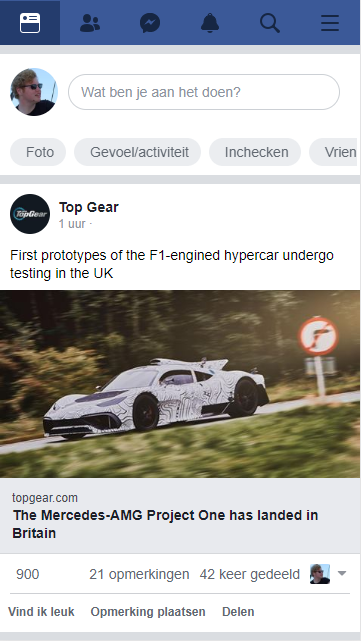
\includegraphics[height=0.4\textheight]{AppVSweb/figures/facebook_web.png}\label{fig:facebookweb}}
  \caption[Facebook native vs Facebook web]{Facebook as an native \textcolor{blue}{(a)} versus Facebook as an web application \textcolor{blue}{(b)}}
  \label{fig:Facebook}
\end{figure*}

%<<<<<<<<<<<<<<<<<<<<<<<<<<<<TO ADD IN INTRODUCTION>>>>>>>>>>>>>>>>>>>>>>>>>>>>
% Deep   description   and critical thinking, evaluation of alternatives, etc.

Around 85\% of Italy's population today use smartphones. 80\% of the total time spent on smartphones is spent on native mobile applications, while only 20\% is spent on mobile Web applications \cite{MobileMark}. Furthermore, 92\% of people consider battery life as one of the significant factors when purchasing a new smartphone. 63\% of the users are unsatisfied with the battery life of their devices, which usually is one day or less, and 66\% would pay more money to extend their phones battery life \cite{BatteryLife_survey}.

Most native applications for the smartphone have a web application as well. For example, in figure \autoref{fig:Facebook} we see the native Facebook application versus the web version. Therefore, this report aims to evaluate whether it is possible to decrease energy consumption by using mobile web applications rather than native mobile applications.The idea that native mobile applications consume more energy is popular in mainstream media. It is relatively easy to find anecdotal proofs of this phenomenon \cite{itworld}. However, although  research has been done into the energy consumption of smartphones in general \cite{pathak2011fine}, mobile applications \cite{balasubramanian2009energy, li2014empirical, couto2014detecting, hao2013estimating} and more specific, into the energy consumption of web apps \cite{thiagarajan2012killed}, very little comparative research has been published between native mobile applications and mobile web applications. Our research will highlight the difference in energy consumption between native and web applications which will provide insight to users on which and to what extent applications types drains their battery, and thus, if they can save battery life by using mobile web applications rather than native mobile applications or the other way around.

An experiment with mobile web applications or native phone applications as independent variable and energy consumption as dependent variable will be carried out. \textit{If we have enough time}, device type (high-end or low-end) as a second independent variable will be added. Five to twenty pairs of the most popular applications will be evaluated using 1 \textit{or more, depending on time}, mobile phones in a controlled environment. To do so,common user actions for each application will be applied on each experimental trial.

%SUGGESTION BY ROBERT: For the critical note, we could make a small remark about using one browser instead of multiple, like this:
A note of caution has to be added, because the experiment is executed with one specific browser (\textit{Google Chrome}), it might be that an experiment with other browsers will yield different results than this research. However, using Chrome, this experiment do cover around 60\% of all browser users worldwide. \cite{Chromestats}
\section{Experiment Definition}\label{sec:definition}
The definition of this experiment is following the GQM (Goal - Questions - Metrics) approach \cite{Basili:1992:SMM:137076}. In this section we define the goal of our experiment, the research questions, and the metrics used to answer those questions.

\subsection{Goal}
\begin{table}[ht]
\centering
\begin{tabular}{||c||} 
\hline
\textbf{Experiment Goal Definition}\\
\hline\hline
Analyze \textbf{native mobile applications \& mobile web applications} \\ 
For the purpose of \textbf{evaluation} \\
With respect to their \textbf{\textcolor{blue}{energy consumption} }\\
From the point of view of \textbf{software users}\\
In the context of \textcolor{blue}{\textbf{the most downloaded applications in Google Play store}}\\ [1ex] 
\hline
\end{tabular}
\caption{Experiment goal of GQM}
\label{tab:goal}
\end{table}
Based on the GQM definition pattern, the experiment goal is defined on Table I:. The goal is to evaluate energy consumption of  native and web applications. The energy consumption of the 5 most popular application pairs will be  monitored, thereafter, if time allows, data from up to 15 pairs of applications will be included. The energy consumption of each trial will be measured 20 times, the mean value of energy consumption for each application will be collected. The browser of choice for web applications is Chrome due to it's popularity\cite{Chromestats}. The popularity of the applications are measured by the number of installations from Google Play. \cite{App_statistics} We are aware that this might give us an biased sample since the most popular applications might have a more or less energy efficient applications relative to general applications. The same reasoning goes for the choice of browser and phone, since Chrome and the phone hardware might be significantly different from other browsers or hardware, this might weaken external validity. \textcolor{blue}{But since we focus on maximizing representativeness and raising the feasibility of the experiment we choose to use the browser and its applications in regard to  popularity.} 
\textcolor{blue}{Finally, the definition of low-end and high-end devices are following the same lines of reasoning as the Mobisoft paper \cite{mobisoft2017}.}

%Further explain why we choose version 6 to be the limit ? 


To summarize, we want to analyze native mobile applications and mobile web applications %..(phone apps and browser apps).. 
for the purpose of evaluation %..(evaluation).. 
with respect to their energy consumption %..(Energy consumption).. 
from the point of view of the software users %..(software developer).. 
in the context of  \textcolor{blue}{ the most downloaded Android applications in Google Play store} %..(Phone usage / thirty phone applications)..?

\subsection{Questions}
Our research embraces 2 research questions:  main research question (RQ1), and 1 additional research question (\textbf{RQ2}). The second question will be explored on the condition that there is enough time.

\textbf{RQ1} - How does energy efficiency differ between native mobile applications and their mobile web counterparts?

To answer to this question, we will have to run the same scenarios on pairs consisting of a native mobile application and its mobile web counterpart. Statistical analysis will be performed to determine whether there is any statistically significant difference.



\textbf{RQ2} - How does the device type affect the difference in energy consumption between native mobile applications and their mobile web counterparts?

To answer this question, we will perform 2 sets of experiments described in \textbf{RQ2}, but one of them has to be on a low-end device, and the other one on a high-end device. Statistical analysis will be performed to determine whether there is any statistically significant difference.


\subsection{Metrics}
We will use the  \textbf{energy \textcolor{blue}{consumption}} to directly answer our research questions. The remaining 3 metrics will supplement our answers with further insight. 
\begin{itemize}
    \item \textbf{Power consumption (W)} - Power consumption of native and web applications while executing the scenario. 	       %measured using Trepn Power Profiler \cite{trepn}.
    \item \textbf{Running time (s)} - total running time of a scenario.
    \item \textbf{Energy consumption (J)} - total energy consumed by running a scenario. Calculated by multiplying the average power consumption and the running time of a scenario.
\end{itemize}
Other metrics would have been possible, for example CPU or memory usage in order to trace the energy consumption of certain applications. However, it would be hard to determine how much the metric would contribute to the energy consumption of the application. Because of that, we decided that these parameters are beyond the scope of this experiment. Some of these metrics however are intrinsically used by the tools that help us find out the metrics we actually do use.
\begin{figure*}[!ht]
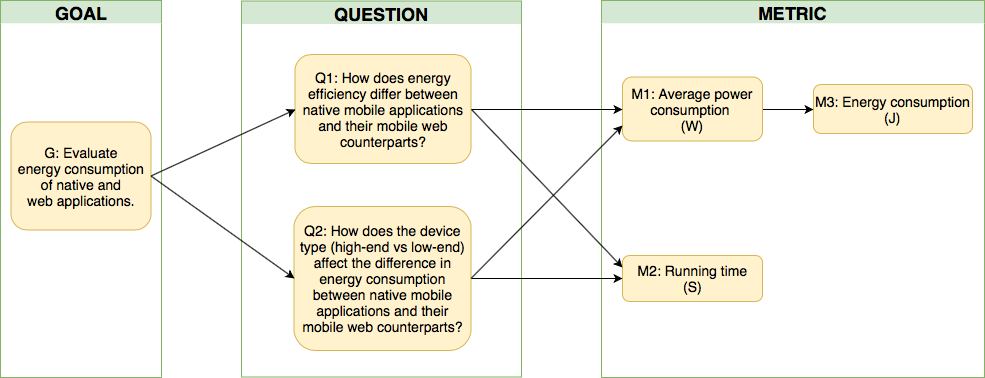
\includegraphics[width=\textwidth]{AppVSweb/figures/GQMtree.png}
\caption{\textcolor{blue}{GQM model hierarchical structure}}
\label{fig:GQMtree}

\end{figure*}
\\To present the experiment idea in a visual way, we picture a GQM tree (\autoref{fig:GQMtree}) based on the elements above.
%\afterpage{\clearpage}


\section{Experiment Planning}\label{sec:planning}

%\begin{itemize}
	%\item Context Selection
	\subsection{Context selection}
The context of the experiment should preferably reflect the real world as much as possible. However, to ensure high external validity within the frames of this project's time scope and feasibility, we decided to narrow our context down to exclusively consider Android devices, specifically the model OnePlus 2. \cite{op2} This model was chosen based on its ability to precisely measure energy consumption and availability to us. Android Runner \cite{androidrunner} is a framework for profiling Android applications, not all devices are compatible with energy profilers used by it under the hood. We also decided to narrow down our browser context to Google Chrome due to its popularity covering 60\% users worldwide.\cite{Chromestats} The definition of the context in our experiment is based on Wohlin et al. dimensions. \cite{wohlin12} There are four dimensions we need to declare.
%The best context to achieve the most general results from experiment is being executed in large, real software projects with professional numbers. However, because of the time and resources limited in reality, and we also have to consider the cost and risks problems. Same situation happened to our experiment too. We limited the context into Android devices %mobile phone model/
	\\
	\subsubsection*{Off-line vs On-line}
	The experiment will be conducted in an \textbf{offline} situation at Vrije Universiteit Amsterdam Green Lab under a controlled environment. There will be no actual users attending the experiment process. As we mentioned in table~\ref{tab:goal}, we choose 20 mobile applications compatible with Android and Google Chrome.
	\\
	\subsubsection*{Students vs Professionals}
	The experiment will be conducted by four researchers (the authors of this paper) with the professional technical guidance (assistant professor Ivano Malavolta). \textcolor{blue}{Since the applications that are considered in this experiment were made by professional application developers renders this experiment as "\textbf{professional}"}.   
	\\
	\subsubsection*{Toy problem vs Real problem}
	% (Paweł's note: This whole subsubsection seems incorrect to me. We're not really fixing any problem; we're checking whether there is a problem. I rewrote this part to reflect it.)
	%The experiment aims at fixing a \textbf{real problem}. In our experiment we work on energy efficiency between native mobile applications and mobile web counterparts. The results could provide insight into alternative energy efficient solutions for users and software developers.
	The experiment aims at researching whether there is a \textbf{real problem}. Our contribution will show whether the common belief about native applications' higher energy consumption can be scientifically proven. A difference in energy consumption can be a good indicator for users caring about battery life of their smartphones. Moreover, if the results indicate a significant difference between native mobile applications and mobile web applications, it could also be an indication for the developers of said applications that research in this area is justified, because there is possibly room for improvement.
	\\
	\subsubsection*{Specific vs General}
	% (Paweł's note: again, we're not going to provide any solutions.)
	For this experiment, a maximum of two Android devices is used: \textit{one} high-end device and \textit{one} low-end device, and web applications will all run on Google Chrome. Therefore, our experiment is \textbf{specific}. However, our conclusions about the relative energy consumption of the two groups of applications at hand could be applicable in a more general context.
	\\
	% justify and evaluate how the experiment should be done, talk about what factors that might influence. offline/online, students/professionals, toy problem/real problem, specific, general 
	%\item Variable Selection
	\subsection{Variable Selection}
	The GQM tree in \autoref{fig:GQMtree} easily visualizes which variables that are being focused on in this experiment. The dependent variable \textit{average energy consumption} is derived from the measurements of \textit{running time} and \textit{energy consumption}. The independent variables are derived from the GQM tree questions (Native \& Web applications) and (High \& Low-end devices).  \textcolor{blue}{As mentioned in \autoref{sec:definition}, the definition of low-end and high-end devices are following the same lines of reasoning as the Mobisoft paper \cite{mobisoft2017}.}


%\limit{2}

  
\subsection{Hypothesis Formulation}
%H0 =  There is no any energy reduction from using phone app or browser. 
% Mean(E:app) = Mean(E:browser)
%\item Subject Selection
\textbf{RQ1} - How does energy efficiency ($\mathcal{E}$)  differ between native mobile applications and their mobile web counterparts?

$H_0^1$ - If we label energy consumption for native applications as $\mathcal{E}_n$ and  energy consumption for web applications as $\mathcal{E}_w$, we can define out null hypothesis as follows:
\newline $H_0^1$        $\mathcal{E}_n = \mathcal{E}_w$\\
Which in natural language means as much as \textcolor{blue}{ "the energy consumption of mobile native applications is the same as the energy consumption of mobile web applications."}

The alternative hypothesis can be mathematically written down as:
\newline $H_a^1$      $\mathcal{E}_n \neq \mathcal{E}_w$\\ 
Which in natural language means that the energy consumption of mobile web applications differs from the energy consumption of their native mobile counterparts.
 
\textbf{RQ2} - How does the device type (high-end vs low-end) affect the difference in energy consumption between native mobile applications and their mobile  web counterparts?

$H_0^2$ - If we label energy consumption for low end devices as $\mathcal{E}_l$ and  energy consumption for high end devices as $\mathcal{E}_h$, we can define out null hypothesis as follows:
\newline $H_0^2$        $\mathcal{E}_l  = \mathcal{E}_h$\\
or "the energy consumption of applications on low-end devices is equal to the energy consumption of applications on high-end devices."

The alternative hypothesis then can be defined as:
\newline $H_a^2$     $\mathcal{E}_l  \neq  \mathcal{E}_h$\\
or "the energy consumption of applications on low-end devices differs from the energy consumption of application on high-end devices."

\textcolor{blue}{ To determine possible interaction effects $\mathcal{I}$ for device and application type following hypothesis needs to be answered: 
Let $\mathcal{I} = (\mathcal{E}_n\mathcal{E}_l - \mathcal{E}_n\mathcal{E}_h)  -  (\mathcal{E}_w\mathcal{E}_l - \mathcal{E}_w\mathcal{E}_h) $  where $\mathcal{E}_n\mathcal{E}_l $ stands for the mean of the group that received $\mathcal{E}_n$ and $\mathcal{E}_l$ and so on. So here we're looking at $(\mathcal{E}_n\mathcal{E}_l - \mathcal{E}_n\mathcal{E}_h)$ which is the effect that device factor is having when we're applying native application. If there is no interaction this should be the same as the device effect is having when we apply web application: $(\mathcal{E}_w\mathcal{E}_l - \mathcal{E}_w\mathcal{E}_h) $. If those are the same then their difference should be 0 so we could use the tests:
\newline $H_0^3$ -  $\mathcal{I} = 0$
\newline $H_a^3$ -  $\mathcal{I} \neq 0$
}
\subsection{Subject Selection}
A pilot study of 5 pairs of applications will be carried out to ensure proper measurement values. The first 5 applications to monitor are Facebook, Twitter, YouTube, Instagram and Google Maps which are chosen from the most popular applications from Google Play. If time allows, the following applications will be monitored: NS, Yelp, WhatsApp, Tinder, AccuWeather, Gmail, Amazon, Ebay, Facebook Messenger, PayPal, Google Play Books, ESPN, Netflix, Duolinguo and Uber. All these applications will be used in  a web browser (\textit{Google Chrome}), and, if time allows, on a high-end phone and a low-end phone. This makes this experiment a \textit{technology-oriented} experiment, as characterized by Wholin et al. \cite{wohlin12}
	%\item Experiment Design
\subsection{Experiment Design}\label{sec:planning-design}
%To answer \textbf{RQ1}, we will have to carry out an paired t-test on a one factor, two treatment design ($1\times2$ design) as \autoref{tab:factor1}.
In order to answer \textbf{RQ1}, we will need one factor, two treatment design with the factor being the type of application. This design is depicted as an $1\times2$ table in \autoref{tab:factor1}. Because we test pairs of applications, we have pairs of results that can best be analyzed with a paired $t$-test, provided that the data is in normal distribution, otherwise the data should be analyzed using a Wilcoxon analysis.

\begin{table}[ht!]
    \centering
    \begin{tabular}{|p{0.4\linewidth}|p{0.4\linewidth}|}
        \hline
        \multicolumn{2}{|c|}{Factor 1: Application Type}\\
        \hline
        \textbf{Native} &  \textbf{Web}\\
        \hline
        Energy consumption measurement (20 times) & Energy consumption measurement (20 times)\\
        \hline
        
    \end{tabular}
    \caption{Design of \textbf{RQ1}}
    \label{tab:factor1}
\end{table}

\textbf{RQ2} however, requires us to analyze two factors, the device type and the application type which both have two treatments each, as depicted in the $2\times2$ table \autoref{tab:factor2}. This requires us to use an factorial ANOVA test as we do not only want to asses the main effect of the factors, but also if there is any interaction between them.
%To answer \textbf{RQ2}, we will have to carry out an factorial ANOVA test on a two factor, two treatment design ($2\times2$ design) as \autoref{tab:factor2}. Two independent variables with 2 levels each requires an factorial ANOVA for analysis. If we decide to only consider one of the independent variables, a T-test will be the choice of analysis. 
The order of the independent trails will be following randomized experiments design. The confidence interval for acceptance of the hypothesis is set to 95\%. 

For the experiment to be meaningful we had to perform the experiment multiple times per application to exclude external factors. The number of repetitions was set to twenty, because this renders small measurement errors futile and gives us more reliable results. 




\begin{table}[!ht]
    \centering
    \begin{tabular}{p{0.2\linewidth}p{0.1\linewidth}|p{0.25\linewidth}|p{0.25\linewidth}|}
        \cline{3-4}
         & & \multicolumn{2}{p{0.5\linewidth}|}{Factor 1: Application Type}  \\ \cline{3-4}
         & & \textbf{Native} & \textbf{Web}\\
        \hline
        \multicolumn{1}{|p{0.2\linewidth}}{\multirow{2}{\linewidth}{Factor 2: Device Type}} &
        \multicolumn{1}{|c|}{\textbf{High}}& Energy consumption measurement (20~times) & Energy consumption measurement (20~times)\\
        \cline{2-4}
        \multicolumn{1}{|c}{}&\multicolumn{1}{|c|}{\textbf{Low}} & Energy consumption measurement (20~times) & Energy consumption measurement (20~times)\\ \hline
    \end{tabular}
    \caption{Design of \textbf{RQ2}}
    \label{tab:factor2}
\end{table}
\subsection{Instrumentation}

For replicability purposes a list of monitoring and data collecting instruments and software are listed and explained below.

\subsubsection*{Objects}
The android device used is an OnePlus 2 \cite{op2}, as this phone is able to provide us with the required data regarding energy consumption. This device can be considered as a high-end device. 

The network infrastructure consists of a WiFi network with a TP-link Archer c2 router \cite{ad7200} using the 802.11ac/n/a standards. The network and router will remain the same throughout the experiment, although the influence on the router settings is limited. The distance from the android device to the router is limited to \textcolor{blue}{at most 5 meters without any obstacles}.
%\subsubsection*{Guidelines} (Checklist documentation)
\subsubsection*{Measurements tools}

We use \textbf{Android Runner} \cite{androidrunner} as a power consumption testing framework. It is equipped with support for different types of experiments (e.g. web-based or native), different profiles (e.g. Trepn \cite{trepn} or Battery-stats \cite{batterystats}), performing arbitrary Android debug commands through Android Debug Bridge \cite{adb}, and executing arbitrary user actions via MonkeyRunner \cite{monkeyrunner}. Android Runner is responsible for fully controlling the experiment and tools used for its execution. 

We use \textbf{Trepn Profiler} \cite{trepn} to monitor power consumption statistics and MonkeyRunner to execute the desired actions for each application in each trial. In each experiment run, Android Runner obtains the execution time from the device itself, executes the actions via Monkeyrunner, and the power consumption via Trepn. It controls when each tool starts and finishes working, and ensures that it is happening in the right order.

\textbf{MonkeyRunner} \cite{monkeyrunner} is a tool for developers which enables to control the connected Android device/emulator. It's capable of installing, launching and manipulating apps, as well as taking screen shots. In this case it is used for executing a series of actions such as browsing pictures, clicking on specific points on the screen and then easily reproduce these actions for each treatment of the independent variables of each application. 

\textbf{R} \cite{team2013r} is an Open source data analysis language which is used for analyzing data and performing statistical tests. To run the scripts written in R we use \textbf{RStudio} \cite{team2015rstudio}, that interprets the R language and is able to show visual representations of the actions performed in R. In our case, it is used to check the data for normality and for running the paired $t$-test and ANOVA test  on our data. 



%\end{itemize}

\section{Experiment Execution}\label{sec:execution}
\subsection{\textcolor{blue}{Overview}}
For each application in the experiment, a trial of common user actions will be executed for each treatment. The native and web application will have an identical navigation pattern or set of actions. The user actions for "Google Maps" could for example be locating a specific point on a map and then search for restaurants in its vicinity. This is done both in the web application and the native application resulting in time and energy consumption for both treatments. Scenarios within application pairs will be executed in random order. 

Testing will be done for up to 20 pairs of applications with batches of 5 applications at a time. This incremental scheme ensures that we can stop the experiment after each each batch of applications, and perform the analysis to ensure that values seems reasonable.

Running the experiment for each application batch will be split into 4 parts: (1) native applications that are executed before their web counterparts, (2) web applications that are executed after their native counterparts, (3) web applications that are executed before their native counterparts, (4) native applications that are executed after their web counterparts.

In case we have enough time to research \textbf{RQ2}, the execution scheme will stay like we have described, but running on a low-end device.

After all execution runs are finished, we are going to preprocess and merge the results using a custom script so that it can be easily used. Later, we will use R to check the assumptions for our data, run the statistical analysis mentioned in \autoref{sec:planning-design}, and generate relevant graphs.

\textcolor{blue}{In our experiment the original web services of the application providers are used. This can influence the validity of the experiment, as we will explain later on.}
%Report about how you plan to conduct your experiment, what data analysis techniques you will use, etc.

%Pairwise comparison with randomized order if time allows.




%\limit{2}

\subsection{\textcolor{blue}{Scenarios}}
\textcolor{blue}{
The descriptions of scenarios for all applications can be found here.}


\textcolor{blue}{\textbf{Google Maps}: Look for "Amsterdam". Go to the directions screen. Choose "Rotterdam" as the starting point. Choose "public transport". Look at the first and the second connection. Look for "Café de Dokter". Show the details. Look through the pictures. Look through the reviews.}

\textcolor{blue}{\textbf{Facebook}: Scroll through the feed down and back up. Search for "Forbes". Look through the photos. Look through the videos.}

\textcolor{blue}{\textbf{Twitter}: Scroll through the feed. Look for "\#RickandMorty". Scroll through videos.}

\textcolor{blue}{\textbf{YouTube}: Look for "Rick Astley Never Gonna Give Up". Watch the first video for 10 seconds. Continue watching it for 30 seconds in fullscreen.}

\textcolor{blue}{\textbf{Instagram}: Scroll through the feed. Go to the stories. Click through them.} 
\section{Results}\label{sec:results}
In this section we will show the results of our analysis. First we will present some descriptive statistics on our data. In the second subsection the results of the paired $t$-test, including the rejection or the acceptance of our hypothesis is presented, and in the remainder there is some further analysis based on the data collected.

%\textcolor{red}{Provide:}
%\begin{itemize}
%\item \textcolor{red}{descriptive statistics}
%\item \textcolor{red}{hypothesis testing}
%\end{itemize}
%\textcolor{red}{Also, provide suitable graphs to illustrate your results.}
\subsection{Descriptive statistics}
\begin{table}[h]
    \centering
\begin{tabular}{|c|c|c|c|}
    \hline
    Application & Average (J) & Minimal (J) & Maximal (J)\\
    \hline
    Google Maps & 80.18 & 47.85 & 110.05 \\
    YouTube & 3.67& 0.48 & 10.09\\
    Facebook & 31.22 & 3.94 &  83.52\\
    Instagram & 8.82 & 4.62 & 14.35\\
    Twitter & 1.92 & 0.25 & 4.67\\
    \hline
    \end{tabular}
    \caption{Average, minimal and maximal energy consumption of running a scenario on native applications}
    \label{tab:native-datapoints}
\end{table}


After collecting the data, the data-set contains a meaningful number of metrics. In \autoref{tab:native-datapoints} we see for each native mobile app the average energy consumption per run, the energy consumption of the run with the least energy consumption and the energy consumption of the run with the largest energy consumption. The same metrics are presented for the mobile web applications in \autoref{tab:web-datapoints}. The difference for each application is presented in \autoref{tab:differences}.

In these basic metrics we can already see some differences between the energy consumption between native mobile applications and mobile web applications. We also see that some applications use way more energy than others (i.e. Google Maps maximally consumes 110.05J on mobile phone, while Twitter only maximally consumes 4.67J on the same device), but also that some applications use more energy as mobile web application than as native mobile application (i.e. Instagram's average energy consumption of running a scenario on web application is 13.36J which is higher than on native application 8.82J), while others use more energy when run as native mobile application than as mobile web application (i.e. Instagram's minimal energy consumption of running a scenario on native application is 4.62J which is higher than on web application 1.90J).

\begin{table}[h]
    \centering
\begin{tabular}{|c|c|c|c|}
    \hline
    Application & Average (J)& Minimal (J)& Maximal (J)\\
    \hline
    Google Maps & 3.85 & 0.35 & 11.76 \\
    YouTube & 2.44 & 0.30 & 8.37 \\
    Facebook & 48.28 & 35.33 & 60.00\\
    Instagram & 13.36 & 1.90 & 35.71 \\
    Twitter & 2.36 & 0.75 & 6.56\\
    \hline
    \end{tabular}
    \caption{Average, minimal and maximal energy consumption of running a scenario on web applications}
    \label{tab:web-datapoints}
\end{table}

\begin{table}[h]
    \centering
\begin{tabular}{|c|c|c|c|}
    \hline
    Application & Difference (native - web) (J) \\
    \hline
    Google Maps & 76.33 \\
    YouTube & 1.23 \\
    Facebook & -17.06  \\
    Instagram & -4.54 \\
    Twitter & -0.44  \\
    \hline
    \end{tabular}
    \caption{Differences in energy consumptions per application}
    \label{tab:differences}
\end{table}

\begin{figure*}[bt]
    \centering
    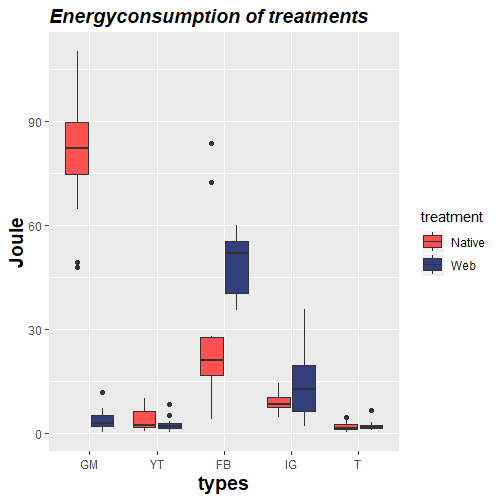
\includegraphics[width=0.5\textwidth]{AppVSweb/figures/Boxplots/Energyconsumption.png}
    \caption{Boxplots of the consumed energy per application}
    \label{fig:Econs}
\end{figure*}

The simple metrics presented in \autoref{tab:native-datapoints} and \ref{tab:web-datapoints} are just a very rough indication, which have to be refined with statistical analysis. In \autoref{fig:Econs} a set of boxplots showing the distribution of measurements for the runs of both the native mobile applications and the mobile web applications. These boxplots show the distribution of data per application, with the horizontal lines being the quartiles of the data, of which the middle one, the second quartile, is the median of the data. The whiskers range from the first and third quartile to the data extremes, as long as they are in 1.5 times the Inter Quartile Range, the outliers are the data points that do not fall within this range.

In this figure a trend is indicated that web applications use more energy than native applications, although not all applications follow this trend \textit{e.g.} YouTube and Google Maps, of which the latter is really deviant from the trend. However, this does not prove anything yet. To give some amount of certainty we need to perform a paired $t$-test if the assumptions for paired $t$-test are met, or a Wilcoxon signed-rank test if the assumptions for the paired $t$-test are not met.

To be able to perform a \textit{t}-test, we need to be certain that the data is in normally distributed. Because of the working of the paired \textit{t}-test, the data we care about are the differences between the pairs of applications. In \autoref{fig:diff_qq} there is a QQ-plot for these differences in energy consumption. This QQ-plot already gives an indication that the data is not normally distributed, as it does not follow a straight line.
% I know the QQ-plot maybe be irrelevant, but we still could use it. Then explain because we did not have time to test enough applications collecting enough data. So the result maybe irrelevant, is that ok?
% - We need a QQ-plot, but we need the right one. The ones already in the folder are probably irrelevant
\begin{figure}[t]
    \centering
    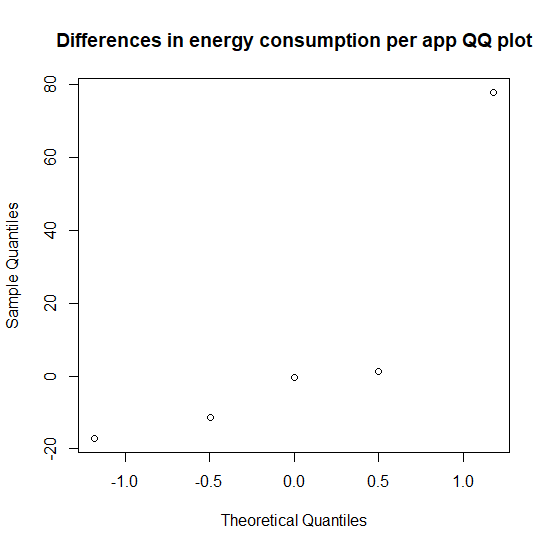
\includegraphics[width=\linewidth]{AppVSweb/figures/QQPlots/diff_qq.png}
    \caption{QQ plot for the differences in average energy consumption per application}
    \label{fig:diff_qq}
\end{figure}
Because the limited number of data-points, it is not obvious to determine whether or not the data is in normal distribution.

To get a more formal indication whether or not the data is normally distributed, a Shapiro-Wilk test for normality \cite{doi:10.1093/biomet/52.3-4.591} was performed on the data. This test returned a \textit{p-value} of 0.0189 for the `signed' differences between pairs, which is not within a 95\% confidence interval to accept normal distribution. When this set is converted to `unsigned' differences, this \textit{p-value} is still 0.01173, which doesn't fall in the 95\% confidence interval to accept the hypothesis that the data is normally distributed either. This means that to draw the right conclusions, we had to perform a non-parametric test on the data, in our case that is the Wilcoxon signed rank test \cite{10.2307/3001968}.


%To be very certain, a Shapiro-Wilk normality test was performed. These resulted in a \textit{p-value} (probability) of $3.3\times 10^{-8}$ for the web values, and $2.03\times10^{-12}$. This means that we need to reject the hypothesis that the data is in normal distribution. %NOTE: what does the data w/o the current Google Maps data? Because that data wildly differs from the other applications.
%\begin{figure}
%    \centering
%    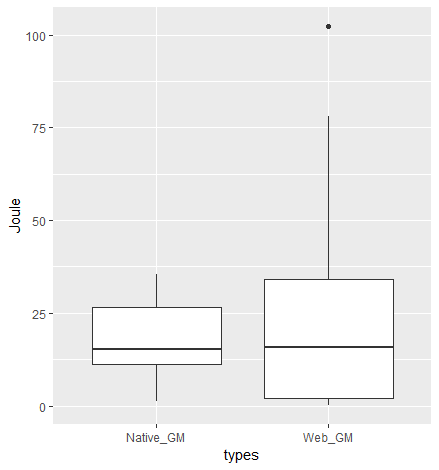
\includegraphics[width=\linewidth]{AppVSweb/figures/Boxplots/GooglemMaps_20.png}
%    \caption{Caption}
%    \label{fig:GMaps_boxplot}
%    %old version
%\end{figure}
% Title missing, need to be modified

%\begin{figure}
%    \centering
%    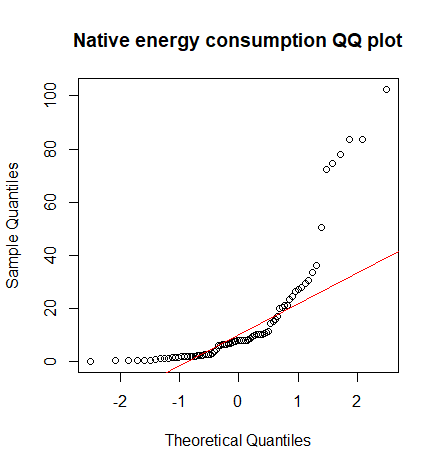
\includegraphics[width=\linewidth]{AppVSweb/figures/QQPlots/Native_energyconsumption_QQ.png}
%    \caption{QQPlot for the distribution for the energy consumption for native applications}
%    \label{fig:Dist2}
%\end{figure}

%\begin{figure}
%    \centering
%    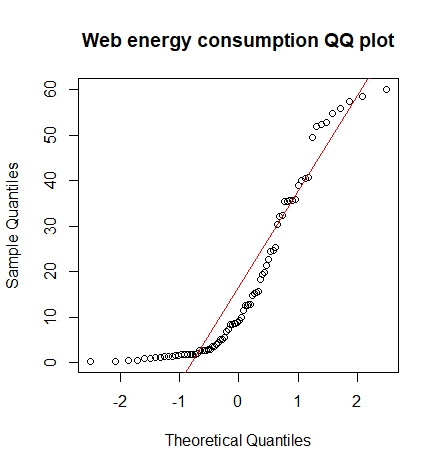
\includegraphics[width=\linewidth]{AppVSweb/figures/QQPlots/web_energyconsumption_QQ.png}
%    \caption{QQPlot for the distribution for the energy consumption for web applications}
%    \label{fig:Dist1}
%\end{figure}
%\begin{figure}
%    \centering
%    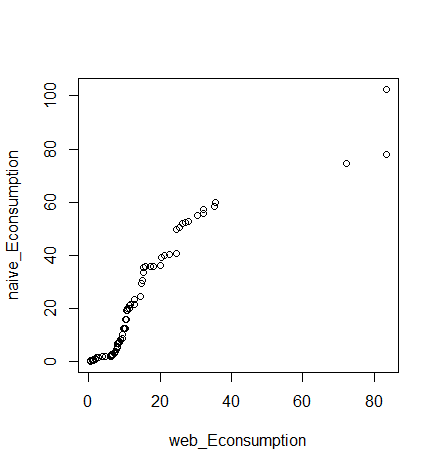
\includegraphics[width=\linewidth]{AppVSweb/figures/QQPlots/QQplot_joulevalues.png}
%    \caption{QQplot for the relative distribution of data}
%    \label{fig:joulevalues}
%\end{figure}


% CHeck for normality in distribution:

% Narmality test for data ( shapiro Wilk test) 
% native values:
% P = 3.27 * e^-8
% web values:
% P = 2.03 * e^-12
% If p < alpha (0.05) then it is NOT normally dist. 
 % + 
% see figures for QQ-plot 
%
\subsection{Hypothesis testing}
\textbf{RQ1} - How does energy efficiency ($\mathcal{E}$)  differ between native mobile applications and their mobile web counterparts?
\\
\newline 
The hypotheses for this research question were as follows:
\newline $H_0^1$        $\mathcal{E}_n = \mathcal{E}_w$ or in natural language: the energy consumption of native mobile applications is equal to the energy consumption of mobile web applications.
\newline $H_a^1$      $\mathcal{E}_n \neq \mathcal{E}_w$, the energy consumption of native mobile applications is not equal to the energy consumption of mobile web applications.

As was treated in the previous subsection, the data did not meet the requirements to perform a paired \textit{t}-test as the data was not in normal distribution. Because of this, the hypothesis was tested using the Wilcoxon signed rank test \cite{10.2307/3001968}. Unlike the t-test, the paired differences do not need to follow a normal distribution but the distribution of each side of the median - must have a similar shape. In other words the distribution of the differences must be symmetrical \cite{Wilcoxon}. Looking at \autoref{fig:LoGPlot} we assume it is quite symmetrical enough. 

\begin{figure}[t]
    \centering
    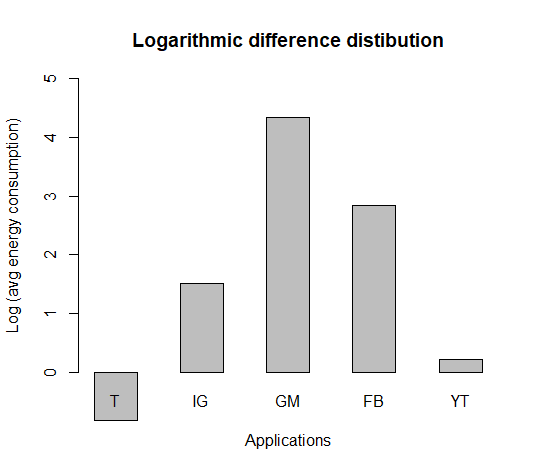
\includegraphics[width=\linewidth]{AppVSweb/figures/LoGPlot.png}
    \caption{Logarithmic distribution of the difference between treatments}
    \label{fig:LoGPlot}
\end{figure}


This test results in an p-value of 1 in an rejection of the null hypothesis that the energy consumption of native mobile applications is equal to the energy consumption of mobile web applications, and thus leads to the acceptance of the alternative hypothesis that the energy consumption of native mobile apps is not equal to the energy consumption of mobile web applications.
%shouldn't we remove the following part, as we didn't have time to dive into this?
\\\newline
Due to the small time-frame of this experiment, we did not have enough time to test our second research question. 

\subsection{Additional statistics}
\begin{figure}[ht]
    \centering
    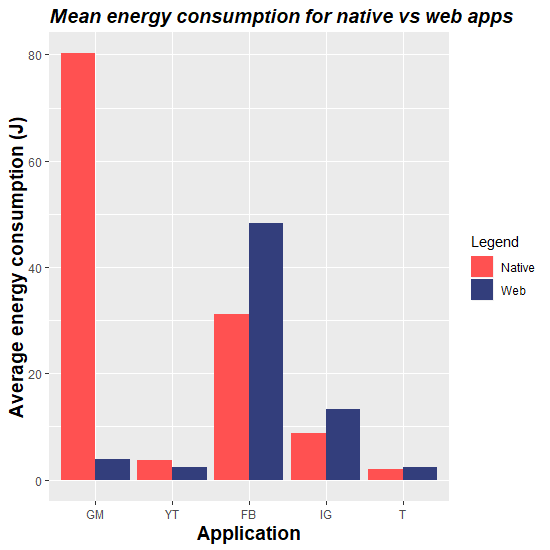
\includegraphics[width=\linewidth]{AppVSweb/figures/Barplot.png}
    \caption{Average energy consumption per application}
    \label{fig:bars}
\end{figure}
In \autoref{fig:bars} the average energy consumption of each application is shown, both as native mobile application as mobile web application. From this plot we see that the difference between native mobile applications and mobile web applications for some applications is limited, there are some applications that do have a significant difference between native mobile applications and mobile web applications. These applications usually have a more than average energy consumption for either native or web or both.

An interesting thing is that for example Google Maps does not only differ from the trend that mobile web applications use more energy than their native mobile counterparts, but does that with a very large difference, as the native mobile application does use quite a lot of energy, while the mobile web application does not use much more energy than for example the YouTube web application. 

A similar kind of result, but the other way around can be seen with the data from Facebook: both the native mobile application and the web application on average use more energy than most applications, but the mobile web application uses a lot more energy than the native mobile application.

Unfortunately, with the data that were collected for this paper it is almost impossible to find out why these differences happen. The reasons for these differences might be an interesting topic for a future research that is more focused on technical details and aimed at the perspective of software developers, but at this moment it goes way beyond the scope of this paper.
%\limit{Open - go deep as you wish}
\section{Discussion}\label{sec:discussion}
In this section we will discuss the implications that the results of our experiment have, and the interpretation of them.

As will be treated in \autoref{sec:threats}, the results collected are not as good as we might hope, as the data have to be derived from other parameters, which harms the validity of this research.

Having said that, it might be interesting to dive deeper in this matter, provided that better ways of measuring energy consumption can be found. Also, when testing more applications, the data might give a better insight in the power consumption of native mobile applications and mobile web applications.

\textbf{RQ1 - How does energy efficiency differ between native mobile applications and their mobile web counterparts?}

Based on the results we concluded, that the energy consumption differs between native mobile applications and mobile web applications. This implies that users might save some battery life by using either native mobile applications or mobile web applications only. Our results overall point to a slight difference in the benefit of native mobile applications. However, because the number of results is very limited, more research is needed to decide if this conclusion holds with a larger number of applications.

Another uncertain part is the question whether or not a certain category of applications can be found that does deviate from the general trend, together with for example Google Maps or YouTube (the former more than the latter). 

\textbf{RQ2 - How does the device type affect the difference in energy consumption between native mobile applications and their mobile web counterparts?}

For Question 2, there is only one device in our experiment OnePlus 2, we could not test the affection of energy consumption between native mobile applications and their web application based on different device types. We could do deeper research in the future.
% Not sure if it is ok saying this way.
\section{Threats To Validity}\label{sec:threats}
%Report about each type of threat to the validity of the experiment, according to the classification discussed in class.
In the following section we identify threats to achieve adequate results. Based on Cook and Campbell \cite{cook1979quasi}, "validity is the extent to which our results are sound and applicable to the real world". There are four types of threats. Their descriptions and the degree of applicability to our experiment are below.

\subsection{Internal Validity}
Internal validity presents causality between the treatment and the outcome of an experiment. It is strongly related to the experiment design and operation. This means that the outcome is directly affected by the treatment. In our experiment, the casual relation of internal validity is between the choice of native mobile applications versus mobile web applications and energy efficiency.

There are four types of internal validity threat and four ways to mitigate the threats.

\textbf{History}: Even though the whole experiment runs on the same device, the device might react differently to different applications. To mitigate this, we keep the environment unchanged as much as possible. Also, there is only one scenario per application pair, and we run each scenario multiple times.

\textbf{Maturation}: The way subjects react to treatments may change over time. This is mitigated by always using a clean application state for each run.

\textbf{Selection}: There is just 1 Android device, OnePlus 2, which may not generalize well. What is more, using only Wi-Fi does not say anything about whether a cellular connection affects relative energy efficiency. We try to use appropriate experiment design to mitigate this threat. For instance, the applications we chose are among the most downloaded applications in Google Play Store, the number of the trials per treatment is same, and the order of the independent trials will follows the randomized experiments design.

\textbf{Reliability of measurements}: Repeating the measurements should yield similar results, and therefore very similar or the same conclusions. The measurement process should also be correct. Unfortunately, we are affected by both of those issues in a way we cannot mitigate. This problem is described in detail in \autoref{sub:softwareproblems}.
% How did TA ANSWER this problem.

%Analyze and identify confounding factors/noise.
%Choose appropriate experiment design.
%Keep environment under control.
%Define representative usage scenarios (if needed)

\subsection{External Validity}
It shows the generalizability of the results and explains how relevant the results are in a wider context. 

There are three types of external validity and two methods to mitigate it.

\textbf{Interaction of selection and treatment}: This threat deals with the selected sample not being representative of the~population of interest. There is a potential risk that the results may not be generalized for all applications. To mitigate this threat, we chose applications that have a high impact on users because they are downloaded very often. This sample is most probably not representative of all applications, but it should be representative of popular applications.

\textbf{Interaction of setting and treatment}: This threat concerns situations where the setting of the experiment does not correspond with reality. Our scenarios, to the best of our knowledge, cover many typical workflows. However, we do not know how representative they are of typical users' actions. To keep the scenarios easily executable in a predictable manner, our workflows do not cover creating content (e.g. taking a picture or typing a longer text) and interacting with other users (e.g. instant messaging).

Unfortunately, due to small differences between the versions of applications, it was not possible to have exactly the same scenarios for both versions of applications. The differences are minimal, and consider how long the total running time and precisely which actions were performed. However, for each pair of applications the scenarios achieve the same goals.

\textbf{Interaction of history and treatment}: This threat is about the experiment being conducted during a specific time which can affect the results, e.g. a specific part of the day or around a special event affecting our subjects. We kept our experiment in an isolated environment and our subjects were applications. The only factors affecting our results could be related to the network unpredictability.
%Use an environment as realistic as possible
%Explicitly define and model your context


\subsection{Construct Validity}
It illustrates the relation between effect and outcome from theory and observation perspectives. The experiment treatment and outcome should reflect on the cause and effect in theory.

There are three types of constructive validity threats and three mitigations.

\textbf{Inadequate preoperational explication of constructs}: This kind of threat usually happens before the execution of the experiment. Therefore, we provided a clear definition of the construct (\autoref{fig:GQMtree}).

\textbf{Mono-operation bias}: This happens when there is only a single object or treatment. The final experiment embraced 5 pairs of applications and our independent variable has 2 treatments, so this threat does not apply to our experiment.



\textbf{Mono-method bias}: This threat is related to a single type of measurements or observations and to the experimenter introducing a bias. In our case using just one application, Trepn, to measure power consumption introduced a bias. This is due to the fact that Trepn was not able to provide precise power consumption values when the device was connected to a computer. This threat is further discussed in \autoref{sub:softwareproblems}.





%Early definition of constructs (GQM)
%Use appropriate experiment design
%Introduce redundancy for cross-checks


\subsection{Conclusion Validity}
Its focus is on statistical correctness and significance between the treatment and the outcome.

There are three types of conclusion validity threats.

\textbf{Low statistical power}: In order to have sufficient data for analysis, we chose as many applications as we were able within the time frame provided by the course schedule. Eventually, we have were able to run tests for 5 pairs of applications.

%\textbf{Violated assumptions of statistical tests}: \todo{Not done yet}

\textbf{Fishing and error rate}: This threat does not apply to our situation, because we are using only one statistical test.

\subsection{Problems with precise measurements}\label{sub:softwareproblems}
During the execution of the experiment we were not able to obtain precise power consumption measurements from Trepn. It was possible to measure correct values, but only when the device was not connected to a computer. This transpired to be a fundamental problem, because without connecting the device to a computer we were not able to control the experiment. This is why all results in this experiment are estimated by Trepn.

We are aware that their values are in many situations unrealistic, but we believe that they are informative to a sufficient degree. Our research questions are not focused on absolute values---it is enough for us to know which values differ significantly between pairs. Trepn being an established tool for measuring power consumption reinforces our trust in the relevance of the results.

Unfortunately, we were not able to use Batterystats, the alternative to Trepn. Android Runner's support for it relied on parsing log and output files of several Android tools. This transpired to be impossible to be done in a reliable fashion. We suspect that this was caused by race conditions related to using those auxiliary Android tools asynchronously. 

This brings us to the point where we doubt whether Android Runner is sufficiently trustworthy when it comes to obtaining precise measurements. In many parts of the source code explicit sleep statements are used to control the flow. Also, as far as we know it has not been tested thoroughly with many devices. We have no way of telling whether this introduced any significant bias.

Related to this is the risk of Android Runner being misconfigured. In the first batch of runs, we used a very short pause between the runs: just 500ms. This turned out to be the cause of an enormous variation between our results. Power consumption between runs for one application differed by a factor of 10. This problem was mitigated by setting the pause between runs to 2 minutes. However, there is no way of telling which wrongly set configuration options had a significant impact on the results.


%Select appropriate tests
%Use only as much significance as needed


 %   \item measurements of power consumption are incorrect (e.g. because it's connected to a computer and it's charging or the device itself is providing inaccurate values)
%    \item using just 1 device doesn't generalize well
%    \item using only Wi-Fi doesn't say anything about cellular data
%    \item our choice of applications can be not representative (because of which applications we chose and the number of applications)
 %   \item our scenarios cover many typical workflows, but maybe those workflows aren't representative
 %   \item workflows don't cover creating content (e.g. taking a picture, typing a longer text) and interacting with other users (e.g. instant messaging)
 %   \item we use only Google Chrome
 %   \item Android Runner may introduce bias, because of possible bugs/misconfiguration
 %   \item there are slight differences in scenarios between native and web due to the applications being a little different - this might introduce a small bias

 
%\limit{1 page}
\section{Conclusions}\label{sec:conclusions}
The goal of our paper was to evaluate energy consumption of native and web applications. In this paper we were able to answer \textbf{RQ1 - How does energy efficiency differ between native mobile applications and their mobile web counterparts?} in an experiment including 5 mobile applications in 2 variants: native and web. Results from statistical analysis showed that there is indeed a difference. Native variants of Google Maps and YouTube consumed more energy than the web variants. Facebook, Instagram, and Twitter had the opposite result.  What is more, due to the lack of time and resources, we could not research \textbf{RQ2 - How does the device type (high-end vs low-end) affect the difference in energy consumption between native mobile applications and their mobile web counterparts?} in our experiment.%should we call the numbers of the research questions here?

There are, however, several important shortcomings of our research that can be addresses in later projects. First of all, we were not able to use precise power consumption measurements. Secondly, our experiment includes only 5 of the most downloaded applications from Google Play Store. Thirdly, as we used only WiFi, we do not know how other network conditions affect the result. Finally, our focus was on the Android ecosystem with Google Chrome, and we cannot draw any conclusions about other ecosystems, e.g. iOS. All of those topics are good starting points for future experiments. Also, another extension of this experiment could be an experiment to find out why there is a difference in energy consumption between native mobile applications and mobile web applications.
 
%One brief paragraph for summarizing the main findings of the report.

%One brief paragraph about the possible extensions of the performed experiment (imagine that other 3 teams will be assigned to the extension of your experiment).  
%
\section{Appendix}\label{sec:appendix}


%\begin{figure}[h!]
%  \centering
%  \begin{subfigure}[b]{0.1\linewidth}
%    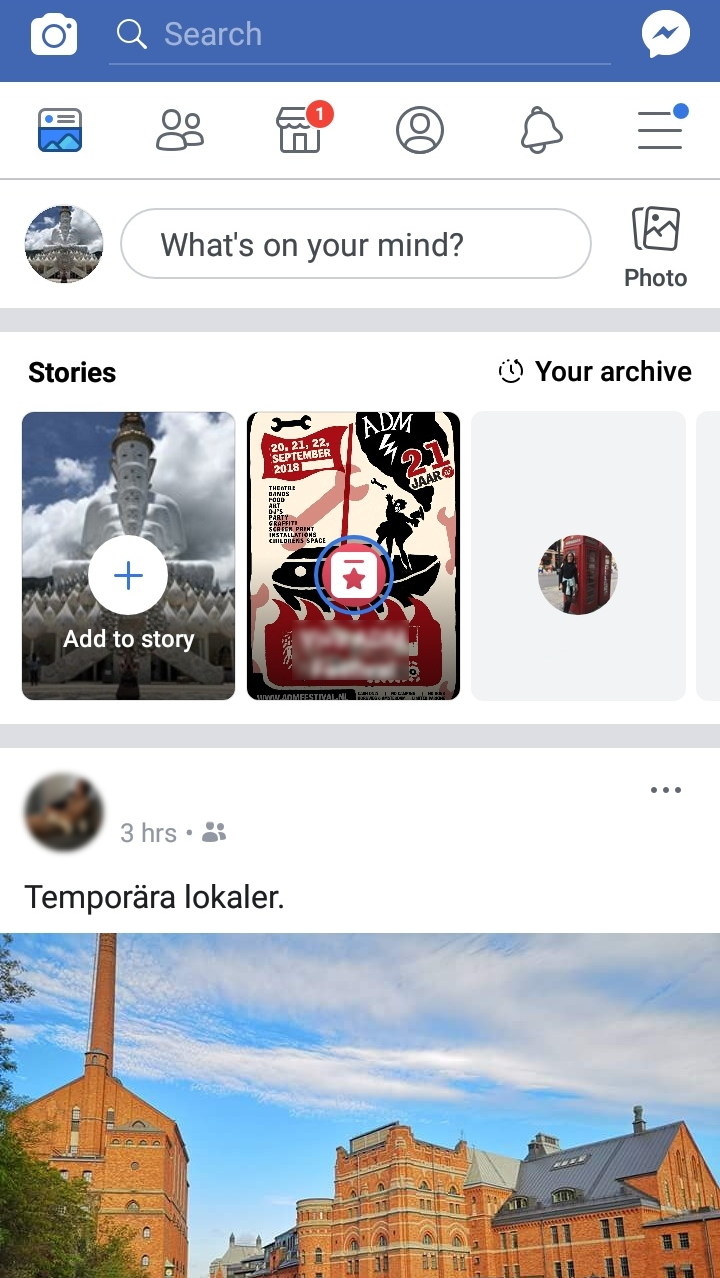
\includegraphics[width=\linewidth]{AppVSweb/figures/Facebook_native.jpg}
%    \caption{Facebook_native.}
%  \end{subfigure}
%  \begin{subfigure}[b]{0.1\linewidth}
%    \includegraphics[width=\linewidth]{AppVSweb/figures/Facebook_web.PNG}
%    \caption{Facebook_web.}
%  \end{subfigure}
%  \caption{Facebook_native and Facebook_web}
%  \label{fig:Facebook}
%\end{figure}
 
\newpage
\bibliographystyle{IEEEtran}
\bibliography{references}

\end{document}
